\section{Power management}
Any commercial camera integrates a flash light, which is turned on in leakage of adequate luminance. I have tried to emulate that behaviour using an high emittance LED. I choose a component able to emit a very cold light: it should be fed with 100 mA at 3V. Having defined the load, then I had to chose the input voltage between two possibilities: 3.3 and 5 volts, both of them directly generated by microcontroller and accessible by means of its own morpho connectors. I thought that the former was too close to the desired output, making the implementation of a converter totally useless. So I decided for 5V as input. Due to the fact that I need of a lower voltage, the straightforward architecture is the Bulk one, whose characteristic is
\begin{equation*}
V_{out} = \dfrac{T_{on}V_{in}}{T_{on}+T_{off}} = \delta V_{in}
\end{equation*}
Another, maybe the most important, feature of a switching regulator is the duty cycle used to drive the NPN transistor's base terminal. First of all I adopted a reasonable period $T = T_{on} + T_{off}$. One of the timer on microcontroller is involved in generating the square wave. It's connected to the Advanced Peripheral Bus (APB) which is synchronized with a clock of 16 Mhz. The timer prescaler has been choosen at 160, so each tick is sensed each 10 $\mu s$. Selecting a period of 100 ticks, the overall period $T$ gets $1 ms$, making any consideration about duty cycle easier. However setting duty cycle isn't so simple, something cannot be taken out from a simple equation.
\begin{figure}[H]
\centering
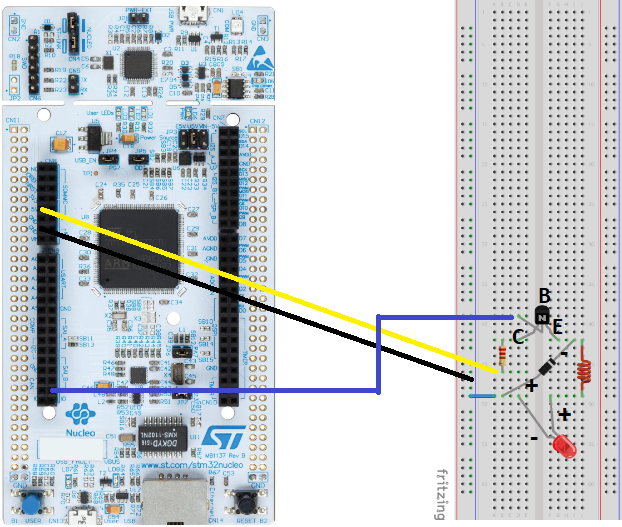
\includegraphics{Immagini/13}
\label{13}
\caption{Connection between MCU and Buck circuit}
\end{figure}

\begin{table}[H]
\centering
\begin{tabular}{p{0.2\textwidth}p{0.4\textwidth}p{0.2\textwidth}}

\textbf{GPIO}&\textbf{Morpho Connector}&\textbf{Description}\\ \hline
PF9 & D63 & TIM14\_CH1 (PWM)\\ 

\hline
\end{tabular}
\caption{Buck: GPIOs involved}
\end{table}

Before showing measurements captured by oscilloscope, I need to state a couple of things. I put a $1K\Omega$ serially the 5V pin in order to avoid overfeeding. It's useless but I was afraid of burning some component: MCU, A2D, camera, resistors, inductor\dots since all of them were connected somehow. Then, few words about the inductor: in the circuit I put $470\mu H$. But, due to the length of $T_{on}$ ($750\mu s$) I would need a much higher one to do not enter in Discontinuos Current Mode. I choose that because it is the biggest I own and have immediate availability. However, everything works and waveforms among the nodes of the circuit seems  to have a compliant shape.

\begin{figure}[H]
\centering
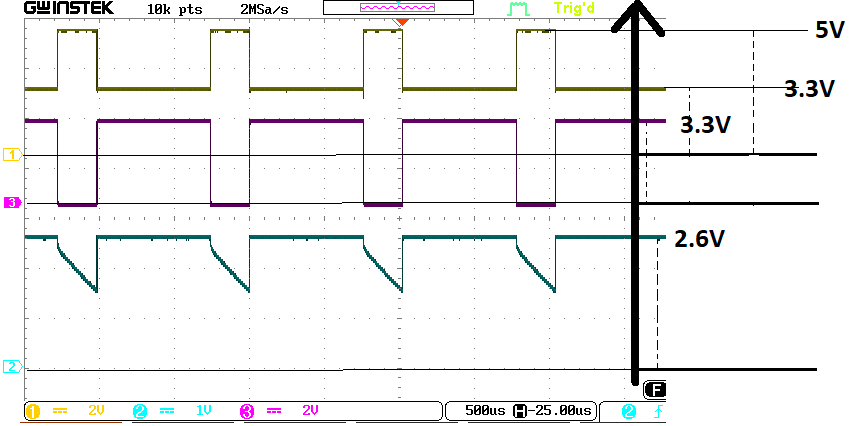
\includegraphics[scale=.7]{Immagini/12}
\label{12}
\caption{From top to bottom: $V_{in}; PWM signal; V_{out}$}
\end{figure}

\begin{figure}[H]
\centering
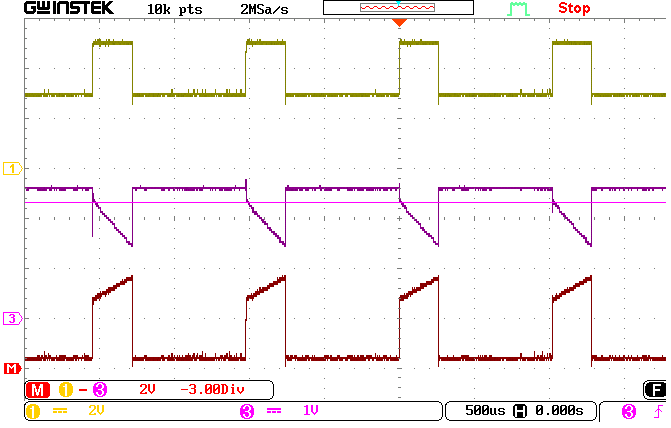
\includegraphics[scale=.8]{Immagini/14}
\label{12}
\caption{From top to bottom: $V_{in}$; $V_A$ of the node where are emitter  diode's cathode and one inductor pin; $V_{out}$, $V_{in}-V_{A}$}
\end{figure}
